\documentclass{article}

\usepackage{CJKutf8}
\usepackage{multicol}
\usepackage[margin=0.5cm]{geometry}
\usepackage{listings}
\usepackage{graphicx}
\graphicspath{ {./img/} }

\title{\textbf{\LARGE {HW2 Branch Predictor Design}}}
\author{學號:0711282 邱頎霖}
\date{}

\begin{document}
\begin{CJK*}{UTF8}{bsmi}
\setlength{\columnsep}{1cm}

\vspace*{-50pt}
    {\let\newpage\relax\maketitle}

\begin{multicols}{2}

\begin{center}
    \section*{INTRODUCTION}
\end{center}

\begin{flushleft}
    \ \ \ \ \ \ 在使用老師所提供的 \ string.c 所得到的\ DMIPS 為\ 0.90342 以此作為初始基準值, \
    首先討論當前\ Aquila 實現分支預測的方式與其缺點,\
    並透過自行以組合語言改寫的\ benchmark 輔助驗證使用\ Two-level Branch Predictor 能更有效提昇效能
\end{flushleft}

\begin{center}
    \section*{ANALYZE}
\end{center}

\begin{flushleft}
    \ \ \ \ \ \ 根據 Aquila 的原始碼,可以知道在\ Aquila 中的分支預測為\ Dynamic branch prediction,\
    以\ 2-bit saturating counter 紀錄\ state machine 狀態且根據預測成功與失敗改變 \ state machine 狀態, \
    原始 Aquila 中以\ 32 個欄位的\ BHT 紀錄\ branch 指令與其狀態機狀態,\
    也就是說當前可以容下\ 32 條指令。\
    我的想法是先嘗試改變\ BHT 的大小觀察 \ DMIPS 是否上升。\newline
    
    \ \ \ \ \ \ 先考慮在沒有分支預測的情況,\
    勢必要到\ pipeline stage 中的 \ execute stage 才可以知道分支結果,\
    一旦需要跳到其他指令處非往下執行就需要做 \ flush,\
    因此即便所有分支預測都錯誤也不過會變成與不使用分支預測一樣的結果,\
    但是一旦預測成功一次便可以省下兩個 \ cycle,\
    因此確認分支預測一定是有好處的。\newline

    \ \ \ \ \ \ 接著考慮 \ BHT 大小對分支預測的影響, 一旦出現不在 \ BHT 的指令,\
    我們就得犧牲掉 \ BHT 中一條指令, 接著將新指令的狀態機初始化後加入 \ BHT 中,\
    雖然初始化預測時也有可能符合正確分支結果,\
    但需要注意的是\ BHT 的意義在於紀錄自己這條分支指令最近的狀態,\
    再根據此狀態去做下一次的預測,\
    因此如果 \ BHT 過小, 將會導致每次都因為空間不夠需要將指令移除與加入,\
    在初始化狀態機時將會導致失去先去獲得的狀態\
    因此我推測一旦將 \ BHT 給縮小將會導致分支預測的效能降低,\ 
    反之如果將 \ BHT 給增加可以增加效能, 但成長曲線會隨之區緩不而會是線性成長
    
\end{flushleft}

\begin{flushleft}
    \ \ \ \ \ \ 因為在拿到老師公告的 \ string.c 前就開始進行測試\
    因此這邊實際測試時將會同時包含我自己在\ HW1 的檔案(\ DMIPS 為\ 0.77)\
    , 與老師提供的共兩個版本(\ DMIPS 為\ 0.90342)。\
    首先我先將\ Aquila 中的分支預測關閉進行測試,\
    根據\ TABLE 1. 可以看到兩個版本都可以看到明顯下降,\
    因此符合我們上述推測的分支預設具有效益。
\end{flushleft}

\begin{flushleft}
    \ \ \ \ \ \ 針對\ BHT size 我選了\ 16,32,64 bit 做測試,\
    原因是先改到 \ 64 bit 後發現\ DMIPS 並沒有上升,\
    查看波形圖後最後發現原因是存放在\ BHT 中的 \ branch 指令數量恰巧為\ 32 條,\
    因此\ BHT 為\ 32 或是 \ 64 將會都是一樣效果。\
    但有趣的是當我把\ BHT size 下降至\ 16 bit 時,\
    自己在\ HW1 的版本出現明顯的下降,\
    老師提供的版本卻不會因此發生變動。\
    當往下調到\ 8 bit 時兩個版本也都沒有因此變低(空間問題不附於\ TABLE 1.)\
    也就是說老師提供的版本在\ 8 bit 與\ 64 bit 的\ BHT 中效果近乎相同。
\end{flushleft}


\begin{center}
    \begin{tabular}{||c c c c c c||} 
     \hline
     Type & Runs & No BHT & 16bit & 32bit & 64bit \\ [2ex] 
     \hline\hline
     T &  1000000 & 0.87832 & 0.90342 & 0.90342 & 0.90342 \\ 
     \hline
     T &  5000000 & 0.87832 & 0.90342 & 0.90342 & 0.90342 \\ 
     \hline
     M & 1000000 & 0.65 & 0.73 & 0.77 & 0.77 \\
     \hline
     M & 5000000 & 0.65 & 0.73 & 0.77 & 0.77 \\
     \hline
    \end{tabular}
\end{center}

\begin{center}
    \small{TABLE 1. DMIPS of different BHT size}\\
    \footnotesize{\ Type 為\ T 為老師提供的版本, \ M 為我自己\ HW1 的版本}\\
    Runs 為\ Dhrystone 中的\ Number of Runs 參數\\
    No BHT 為將分支預測關掉的測試, 16,32,64 bit 分別為代表\ BHT 大小
\end{center}

\columnbreak
% another column

\begin{center}
    \section*{WEAKNESS OF BINMODAL PREDICTION}
\end{center}

\begin{flushleft}
    \ \ \ \ \ \ Bimodal prediction 雖然容易實做且對效能的提昇有著不錯的效果,\
    但我們仍然可以刻意的找出對\ Bimodal prediction 不友善的指令執行方式。\
    首先,\ Aquila 中\ Bimodal prediction 的狀態機初始狀態為 \ Strongly taken,\
    因此如果我們故意使每次真正分支結果與預測相反如\ TABLE 2. 所示,\
    將可以得到\ hit rate 為\ 0\% 的預測器。\
    但這個想法過於完美,\
    不可能真正做出一個讓當前\ bimodal prediction hit rate 為\ 0 的程式,\
    但仍可以以這個想法作為核心改寫\ Dhrystone 內容,\
    盡量使得當前\ bimodal prediction 預測失敗次數增高,\
    並以\ Hit 次數,\ Miss 次數, 執行時間三者因素對當前\ Aquila 的\ branch predictor 與\ two-level branch predictor 的比較。\
\end{flushleft}

\begin{flushleft}
\begin{tabular}{||c c c c c c c c c||} 
    \hline
     & 1 & 2 & 3 & 4 & 5 & 6 & 7 & 8 \\ [1.5ex] 
    \hline\hline
    Real T/NT &  NT & NT & T & T & NT & NT & T & T  \\ 
    \hline
    Predict  &  T & T & NT & NT & T & T & NT & NT  \\ 
    \hline
    Hit/Miss & M & M & M & M & M  & M & M & M \\
    \hline
\end{tabular}
\end{flushleft}

\begin{center}
    \small{TABLE 2. Weakness example}\\
\end{center}

\begin{flushleft}
    \ \ \ \ \ \ 上述想法的實現方式大致如下,\
    大致邏輯不變動的情況下我以組合語言實現,\
    避免以高階語言選寫時遭到編譯器優化,\
    其中中間段落的部份即是全部\ Miss 的情況,\
    當\ bimodal prediction 第一次遇見此\ if statment 時,\
    將會初始化為\ Strongly taken,\
    重複在\ TABLE 2. 中的動作不斷\ Miss,\
    而唯一造成\ Hit 增加的因素為外迴圈次數,\
    因此如果我們在內迴圈多放幾次或是減少外迴圈次數將會有效率提高\ Miss/Hit 比重,\
    FIG. 1. 展示了隨著外迴圈次數增長,\ Hit 與\ Miss 差異將逐漸增大的趨勢
\end{flushleft}

\begin{center}
    \begin{lstlisting}[
        basicstyle=\footnotesize, 
    ]
        for(i=0;i<Number of Runs;i++){
            int j=0;
            int flag=0;
            for(;j<4;j++){
                if(j>1)flag=1;
            }
        }
    \end{lstlisting}
\end{center}

\begin{center}
    \footnotesize CODE. 1. Example code for exploit weakness of bimodal prediction
\end{center}

\begin{flushleft}
    \begin{center}
        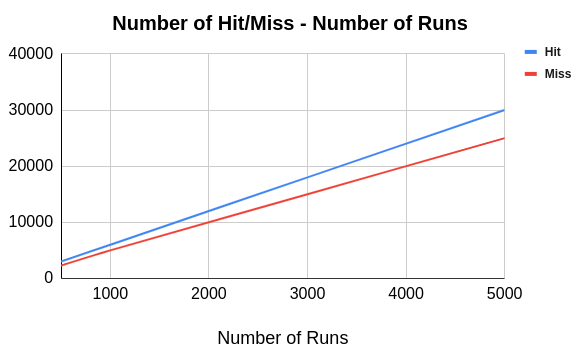
\includegraphics[width=9cm]{hitmiss}\\
        \footnotesize FIG. 1. Number of Hit versus Number of Miss
    \end{center}
\end{flushleft}


\newpage

\begin{center}
    \section*{IMPLEMENTATION}    
    \subsection*{rescheduling}
\end{center}

\end{multicols}

\end{CJK*}
\end{document}